\addsection{Interface}
\begin{figure}[tbh]
  \centering
  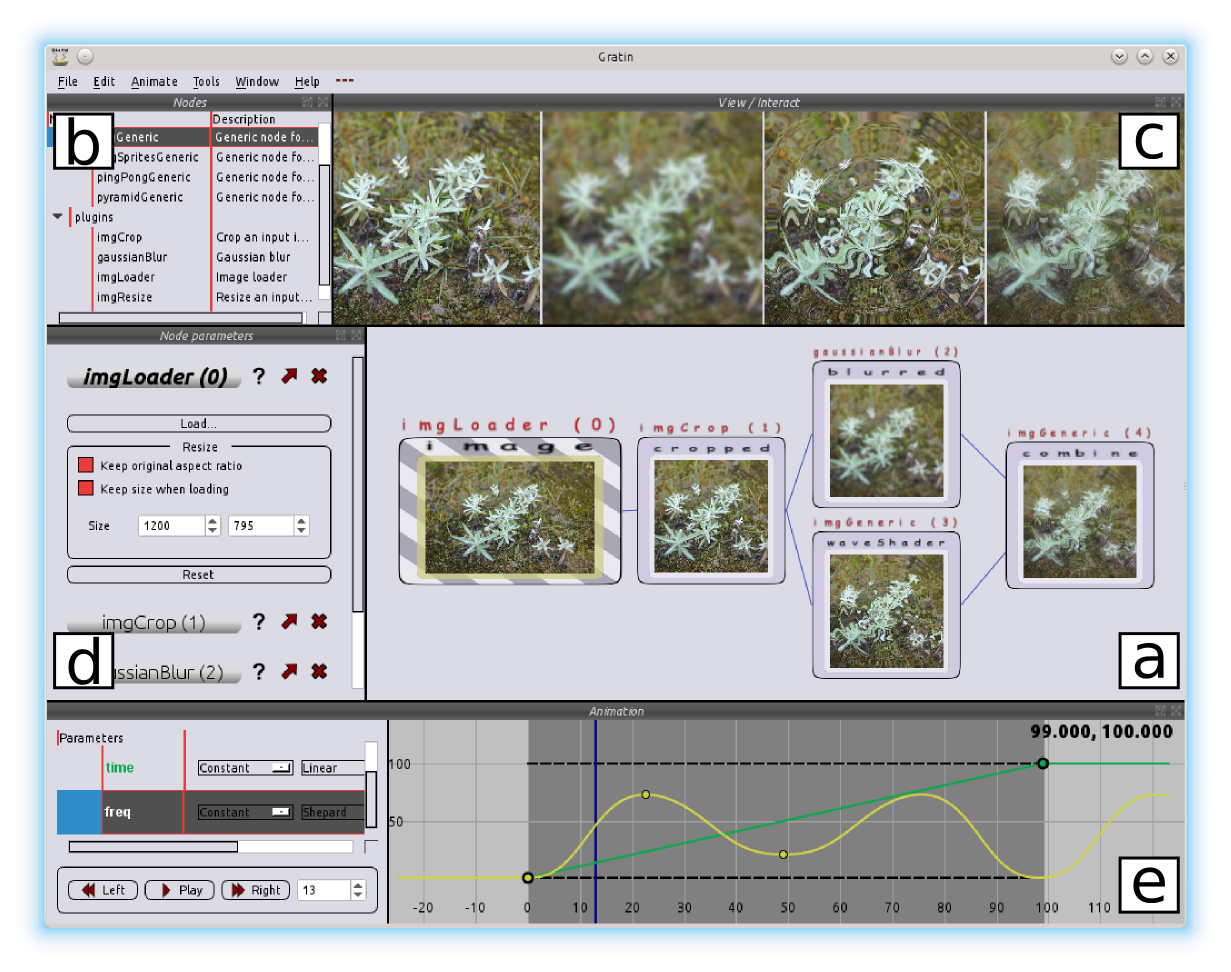
\includegraphics[width=\linewidth]{imgs/interface.png}
  \caption{\label{fig:interface}Interface of Gratin. (a) Graph
    visualization. (b) List of available nodes. (c) Node viewer. (d)
    Node interfaces. (e) Animation parameters and curves.}
\end{figure}

\noindent As shown in Figure~\ref{fig:interface}, the interface of our system
is composed of five main panels. The pipeline panel (a) where one can
interactively add, connect, disconnect, copy or paste nodes.  Node
outputs are visualized in real-time inside the interface.  All available nodes
are stored in user-defined directories and automatically loaded in the
node tree (b) at initialization.  The viewer (c) permits to display
particular node outputs and manipulate them via keyboard or mouse
events.  Each node has its own user-interface that can be displayed
and manipulated via a list of widgets (d).  Any node parameter may be
keyframed and interpolated via control curves in the animation panel
(e).

\newpage 

\addsubsection{Menu and global shortcuts}
\addparagraph{File menu}
\begin{itemize}
  \setlength\itemsep{0cm}
\item New (ctrl+n): clear everything. 
\item Open (ctrl+o): open an existing pipeline.
\item Save (ctrl+s): save/resave the current pipeline.
\item Save as: save the current pipeline in a new file.
\item Exit: quit the application. 
\end{itemize}

\addparagraph{Edit menu}
\begin{itemize}
 \setlength\itemsep{0cm}
\item Copy (ctrl+c): copy selected nodes inside the pipeline.
\item Paste (ctrl+v): paste selected nodes inside the pipeline.
\item Select all (ctrl+a): select/unselect all the nodes of the pipeline.
\item Reload: does nothing (only for debugging new implemented nodes).
\end{itemize}

\addparagraph{Animate menu}
\begin{itemize}
 \setlength\itemsep{0cm}
\item Play (p): start the animation. 
\item Stop (shift+p): stop the animation.
\item Next frame (shift+right): compute and show the next frame.
\item Previous frame (shift+left): compute and show the previous frame.
\item First frame (shift+up): compute and show the first frame.
\item Last frame (shift+down): compute and show the last frame.
\item Anim settings: choose the number of frames and the framerate. 
\end{itemize}

\addparagraph{Tools menu}
\begin{itemize}
 \setlength\itemsep{0cm}
\item Group (ctrl+g): group selected nodes (only if they form some directed acyclic graphs).
\item Ungroup (ctrl+shift+g): ungroup the selected node (only if the node is a group).
\item Export node output (ctrl+w): save a node output image (if an output is selected). 
\item Export node output animation (ctrl+shift+w): save all frames of a node output image (if an output is selected). 
\item Add node to list: if a node has been customized, this option allows the user to add the node inside the list of available nodes (panel b). The user has to choose a unique ID, a version, a name, a description and a help string that will be used for the new node. He also has to choose, in the list of available directories, the one in which the node will be saved. 
\item Manage node paths: allows the user to add or remove directories in which Gratin will look for new nodes when launched. This action needs a restart of Gratin. 
\end{itemize}

\addparagraph{Tools menu}
\begin{itemize}
 \setlength\itemsep{0cm}
\item Window/show-hide: show or hide panels (b), (c) and (d). 
\item Window/zoom: zoom/resize pipelines and images in panels (a) and (c).
\end{itemize}

\addparagraph{Help menu}
\begin{itemize}
 \setlength\itemsep{0cm}
\item Help: show the help widgets for all available nodes. 
\item About: display some information about Gratin. 
\end{itemize}

\addsubsection{Pipeline panel (a)}
\addparagraph{Summary of controls}
\begin{itemize}
 \setlength\itemsep{0cm}
\item Left click on a node: select it. If the click was done on an image, this action also selects the corresponding output inside the node. 
\item Double left click on a node: display its interface (panel d). 
\item Left click on the background : unselect all.
\item Left click, drag, drop on the background: select multiple nodes.
\item Right click, drag, drop on the background: move the scene.
\item Left click on an output, drag and drop on an input: create a connection. 
\item Wheel/middle click: zoom in/out.
\item Left click on a selected nodes, drag and drop: move selection.
\item Press space: add/remove a selected node output inside the viewer (panel c)
\item Press suppr: remove selection from the graph.
\end{itemize}

\addsubsection{Node panel (b)}
\noindent The node panel contains the tree of available nodes that can be added and combined inside the pipeline. A small description is also shown for each node. A double left click on a node will automatically insert it inside the graph. 

\vspace{0.5cm}
\addsubsection{Viewer panel (c)}
\addparagraph{Summary of controls}
\begin{itemize}
 \setlength\itemsep{0cm}
\item Left click on an image: select the corresponding node. 
\item mouse/keyboard on top of a selected node: interact with the node (depends on the node).
\item Left click on the background / press esc: unselect everything.
\item Right click, drag, drop on the background: move the scene.
\item Wheel/middle click: zoom in/out. 
\item Press suppr: remove selected node from the viewer. 
\item Press ctrl+right: move selected node to the right.
\item Press ctrl+left: move selected node to the left.
\end{itemize}

\addsubsection{Node interface (d)}
\begin{figure}[tbh]
  \centering 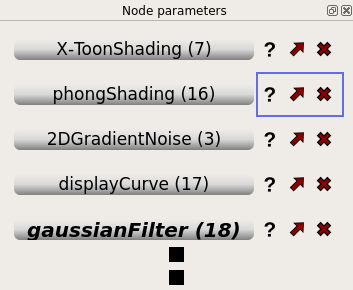
\includegraphics[width=0.4\linewidth]{imgs/node-param.png} 
  \caption{\label{fig:node-param}Each
  node interface is displayed as a list of widgets in the panel d. }
\end{figure}
\noindent The panel d contains a list of node interfaces opened by the user (via a double click on a node), as shown in Figure~\ref{fig:node-param}. Each widget thus contains parameters specific to each node as well as 3 buttons (as shown in the blue square):
\begin{itemize}
 \setlength\itemsep{0cm}
\item a help button (showing a small widget containing the documentation of this particular node),
\item a detach button (detach the window - useful when programming inside the interface),
\item a close button that removes this interface from the list (simply double-click again on the node to show it again). 
\end{itemize}
%
\begin{figure}[tbh]
  \centering 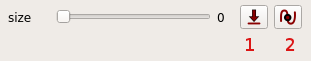
\includegraphics[width=0.4\linewidth]{imgs/one-param.png} 
  \caption{\label{fig:one-param}A keyframable parameter.}
\end{figure}
Each parameter contained in the node interface might be animated using keyframed curves. A keyframed parameter can be easily recognized by its associated 2 buttons, as shown in Figure~\ref{fig:one-param}:
 \begin{enumerate}
 \setlength\itemsep{0cm}
\item create a keyframe at the current frame with the chosen value inside the interface. 
\item Add the parameter inside the animation panel (d) in order to control its curve(s). 
\end{enumerate}


\addsubsection{Animation panel (e)}
\begin{figure}[tbh]
  \centering 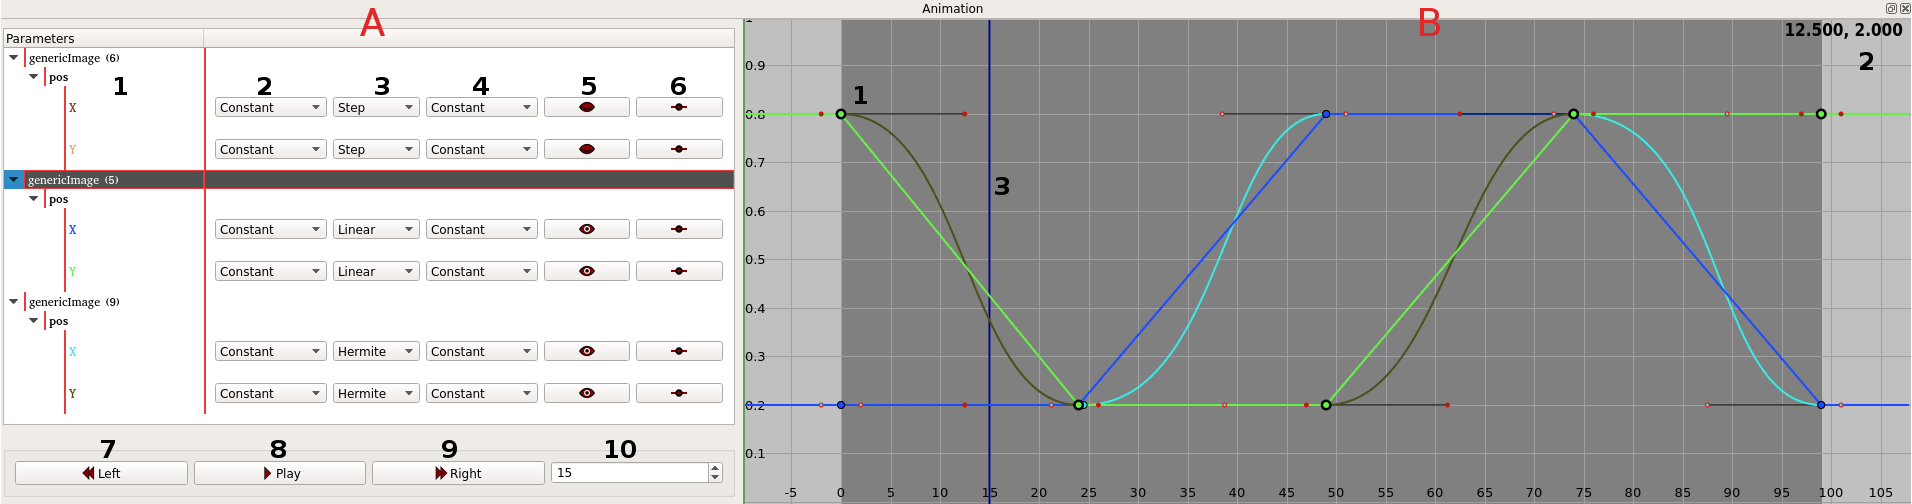
\includegraphics[width=1\linewidth]{imgs/anim-widget.png} 
  \caption{\label{fig:anim-widget}The animation panel}
\end{figure}
\noindent The animation panel is composed of 2 main widgets, as shown in Fig.~\ref{fig:anim-widget}. The first one (A) contains the list of parameters currently edited by the user, their options and the player. The second one (B) shows the corresponding keyframed curves that can be edited directly. 

\addparagraph{A: list of parameters}
\begin{enumerate}
 \setlength\itemsep{0cm}
\item parameters are displayed in a tree widget, containing the node name (root), the parameter name and each of its components. 
\item control the behavior of the curve before the first control point (see Fig.~\ref{fig:curves}). 
\item control the type of interpolation used in-between control points (see Fig.~\ref{fig:curves}). 
\item control the behavior of the curve after the last control point (see Fig.~\ref{fig:curves}). 
\item show/hide the curve in widget B.
\item clear all control points for this curve.
\item (shift+up) place the current frame at the beginning of the animation.
\item (p and shift+p) play/stop the animation 
\item (shift+down) place the current frame at the end of the animation.
\item show and select the current frame.
\end{enumerate}
Available curve behaviors and types are summarized in Fig.~\ref{fig:curves}. 

\begin{figure}[htb]
 \centering
\begin{tabular}{@{} c @{\hspace{4pt}} c @{\hspace{4pt}} c @{\hspace{4pt}} c @{\hspace{4pt}} c @{\hspace{4pt}} c @{}}
 & \tiny{Constant} & \tiny{Linear} & \tiny{Repeat} & \tiny{Offsetted} & \tiny{Mirrored}\\
 \rotatebox[origin=c]{90}{\rlap{\tiny{Linear}}}&
 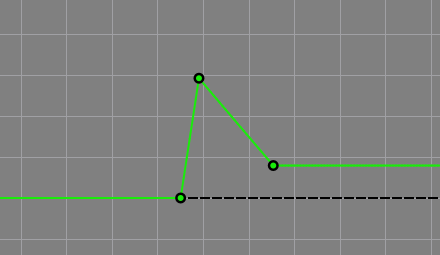
\includegraphics[width=0.19\linewidth]{imgs/kf01.png}&
 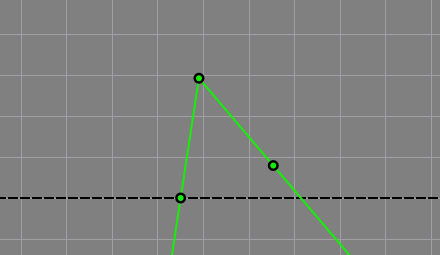
\includegraphics[width=0.19\linewidth]{imgs/kf06.png}&
 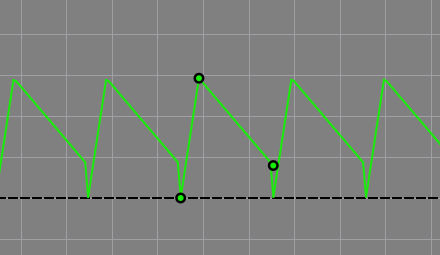
\includegraphics[width=0.19\linewidth]{imgs/kf11.png}&
 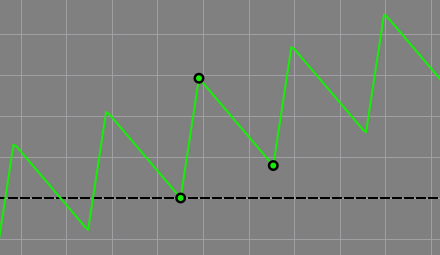
\includegraphics[width=0.19\linewidth]{imgs/kf16.png}&
 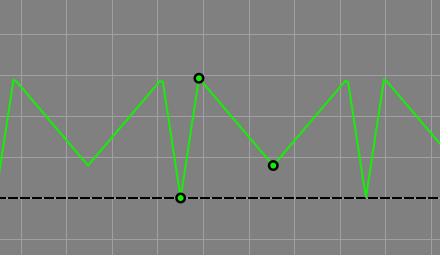
\includegraphics[width=0.19\linewidth]{imgs/kf21.png}\\
 \rotatebox[origin=c]{90}{\rlap{\tiny{Step}}}&
 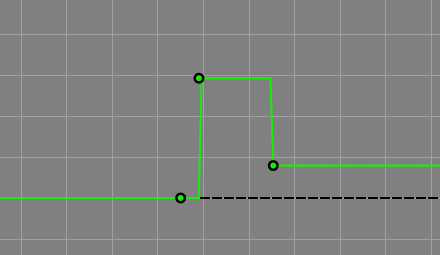
\includegraphics[width=0.19\linewidth]{imgs/kf02.png}&
 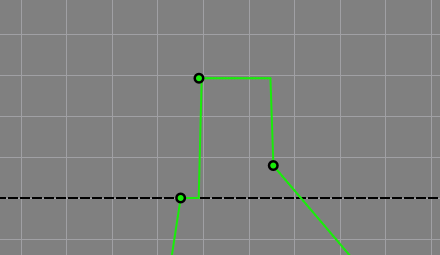
\includegraphics[width=0.19\linewidth]{imgs/kf07.png}&
 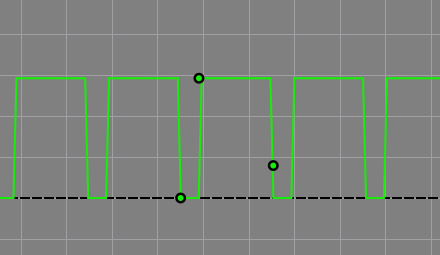
\includegraphics[width=0.19\linewidth]{imgs/kf12.png}&
 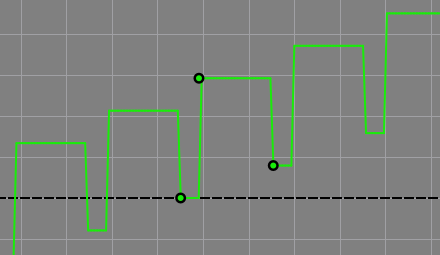
\includegraphics[width=0.19\linewidth]{imgs/kf17.png}&
 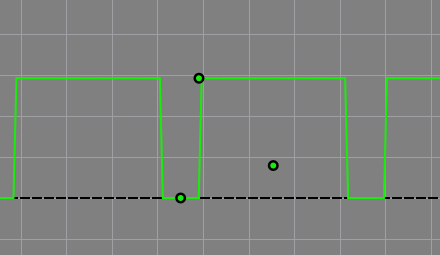
\includegraphics[width=0.19\linewidth]{imgs/kf22.png}\\
 \rotatebox[origin=c]{90}{\rlap{\tiny{Shepard}}}&
 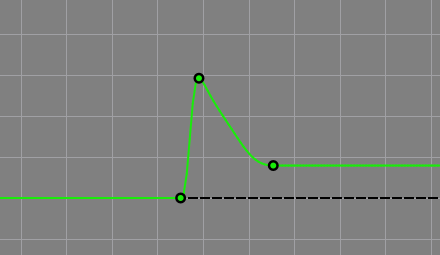
\includegraphics[width=0.19\linewidth]{imgs/kf03.png}&
 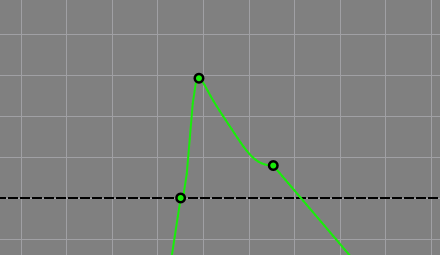
\includegraphics[width=0.19\linewidth]{imgs/kf08.png}&
 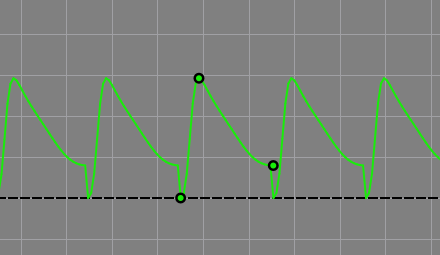
\includegraphics[width=0.19\linewidth]{imgs/kf13.png}&
 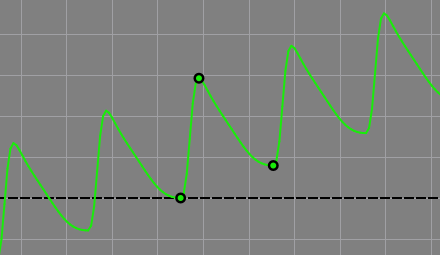
\includegraphics[width=0.19\linewidth]{imgs/kf18.png}&
 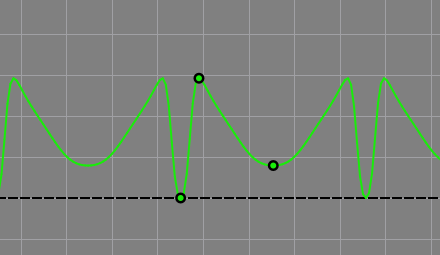
\includegraphics[width=0.19\linewidth]{imgs/kf23.png}\\
 \rotatebox[origin=c]{90}{\rlap{\tiny{Spline}}}&
 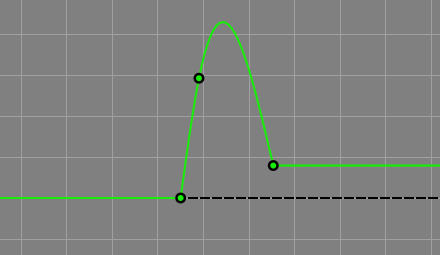
\includegraphics[width=0.19\linewidth]{imgs/kf04.png}&
 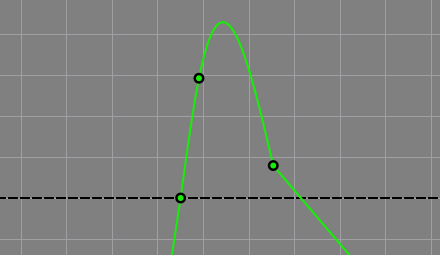
\includegraphics[width=0.19\linewidth]{imgs/kf09.png}&
 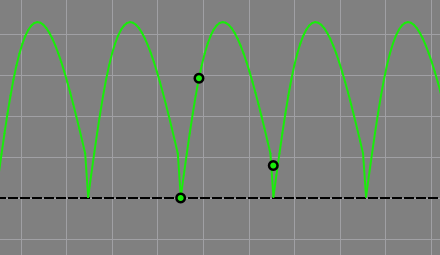
\includegraphics[width=0.19\linewidth]{imgs/kf14.png}&
 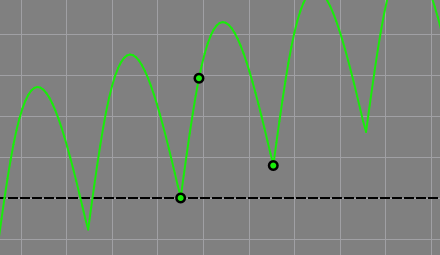
\includegraphics[width=0.19\linewidth]{imgs/kf19.png}&
 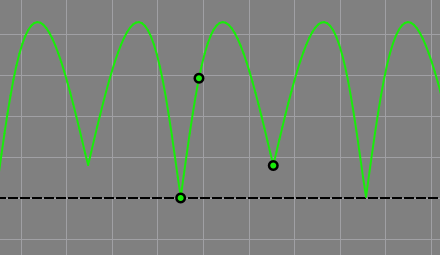
\includegraphics[width=0.19\linewidth]{imgs/kf24.png}\\
 \rotatebox[origin=c]{90}{\rlap{\tiny{Hermite}}}&
 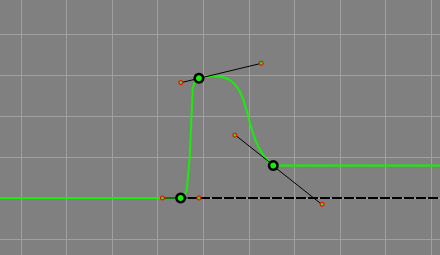
\includegraphics[width=0.19\linewidth]{imgs/kf05.png}&
 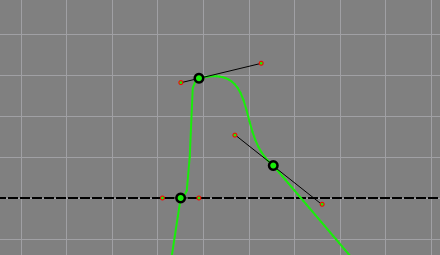
\includegraphics[width=0.19\linewidth]{imgs/kf10.png}&
 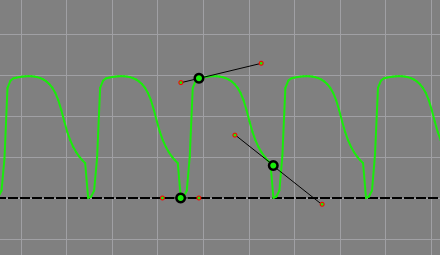
\includegraphics[width=0.19\linewidth]{imgs/kf15.png}&
 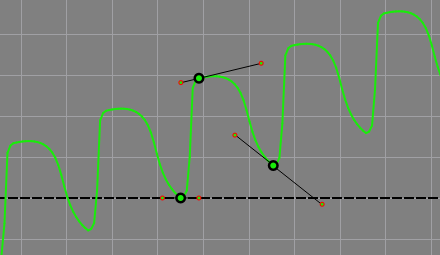
\includegraphics[width=0.19\linewidth]{imgs/kf20.png}&
 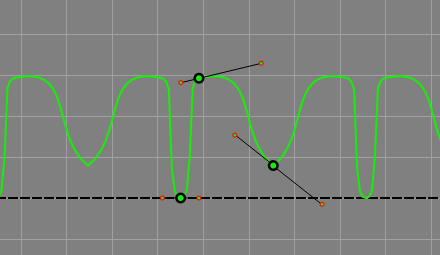
\includegraphics[width=0.19\linewidth]{imgs/kf25.png}
 \end{tabular}
\caption{\label{fig:curves}
Curve types and behaviors obtained with three control points. 
The y-axis shows the types of interpolation implemented in our system. 
The x-axis shows the modes controlling the behavior of the curves before and after the first and last control points. }
\end{figure}

\addparagraph{B: curve edition}

\noindent All selected curves can be visualized and edited in widget B. Control points are displayed with small dots (1). Their positions are displayed on the top right corner (2). The current frame is also displayed with a blue line (3). Here is a summary of the controls in this widget:
\begin{itemize}
 \setlength\itemsep{0cm}
\item Left click on the frame bar and drag: modify the current frame. 
\item Left click on a control point: select the corresponding curve. 
\item Left click on a control point and drag: modify the position of the control point. 
\begin{itemize}
 \setlength\itemsep{0cm} 
 \item +ctrl: use big steps to control the position. 
 \item +shift: use small steps to control the position. 
\end{itemize}
\item Ctrl+right click on the background: add a control point to the selected curve.
\item Ctrl+middle click on a control point: remove the control point from the selected curve.
\item Right click on the background: move the scene.
\item Wheel: zoom in/out.
\item Ctrl+wheel/middle click and drag horizontally: horizontal scaling.
\item Shift+wheel/middle click and drag vertically: vertical scaling.
\end{itemize}
